\label{cha:performance_protein}
The following chapter is dedicated to evaluate the different machine learning and feature engineering methods on
the target compounds. For each protein the top two approaches are evaluated further.

\subsection{Acetylcholinesterase}
The following table presents the results of the different machine learning algorithms on the various
test-sets. The ROC curves for the top two performing configurations can be found at \ref{fig:ache_baseline_rf_roc} and \ref{fig:ache_smote_rf_roc}
respectively. The confusion matrices can be found at \ref{fig:ache_baseline_rf_conf} and \ref{fig:ache_smote_rf_conf}.
The scoring functions achieved an accuracy score of 81.06\% on the test-set.
\begin{table}[H]
    \begin{center}
        \caption{Acetylcholinesterase performance test-set}
        \begin{tabular}{lrrrrr}
            \toprule
            Name             & ACC    & FPR    & AUC    & EF     & REF     \\
            \midrule
            baseline\_rf     & 0.8106 & 0.3285 & 0.7992 & 1.4161 & 92.6829 \\
            fe\_smote\_rf    & 0.8007 & 0.3358 & 0.7894 & 1.4046 & 91.4634 \\
            fe\_smote\_nn    & 0.7708 & 0.2993 & 0.7650 & 1.4102 & 82.9268 \\
            baseline\_nn     & 0.7674 & 0.2920 & 0.7626 & 1.4134 & 81.7073 \\
            fe\_rf\_per\_knn & 0.7575 & 0.4307 & 0.7420 & 1.3172 & 91.4634 \\
            baseline\_knn    & 0.6844 & 0.5766 & 0.6629 & 1.1966 & 90.2439 \\
            fe\_rf\_mdi\_knn & 0.5515 & 0.4307 & 0.5530 & 1.0987 & 59.8639 \\
            \bottomrule
        \end{tabular}
    \end{center}
\end{table}

\begin{figure}[H]
    \begin{center}
        \caption[]{Baseline random forest confusion matrix}
        \label{fig:ache_baseline_rf_conf}
        \includegraphics[height=8cm]{ache/baseline_rf_conf.jpg}
    \end{center}
\end{figure}
The confusion matrix for the baseline random forest model shows that it performs relatively well as the diagonal values(152, 92) are proportionally high
when compared to the rest of the values. The model is more likely to predict a false positive than it is predicting a false negative.  

\begin{figure}[H]
    \begin{center}
        \caption[]{SMOTE random forest confusion matrix}
        \label{fig:ache_smote_rf_conf}
        \includegraphics[height=8cm]{ache/fe_smote_rf_conf.jpg}
    \end{center}
\end{figure}
The matrix shows that the model is a fractionally less likely to predict a false negative when compared to \ref*{fig:ache_baseline_rf_conf}. However, the accuracy is marginally worse.  

\begin{figure}[H]
    \begin{center}
        \caption[]{Baseline random forest ROC curve}
        \label{fig:ache_baseline_rf_roc}
        \includegraphics[height=8cm]{ache/baseline_rf_roc.jpg}
    \end{center}
\end{figure}
The ROC curve leans towards the top left corner, which indicates a good performance. It is closer to a perfect 1.0 than it is to the random threshold of 0.5.

\begin{figure}[H]
    \begin{center}
        \caption[]{SMOTE random forest ROC curve}
        \label{fig:ache_smote_rf_roc}
        \includegraphics[height=8cm]{ache/fe_smote_rf_roc.jpg}
    \end{center}
\end{figure}
The appearance of the ROC curve signifies a good discriminative performance, although the AUC score of 0.79 indicates that the performance is not as good as \ref*{fig:ache_baseline_rf_roc}.

\subsection{Cyclooxygenase 1}
The following table presents the results of the different machine learning algorithms on the various
test-sets. The ROC curves for the top two performing configurations can be found at \ref{fig:cox1_baseline_rf_roc} and \ref{fig:cox1_smote_rf_roc}
respectively. The confusion matrices can be found at \ref{fig:cox1_baseline_rf_conf} and \ref{fig:cox1_smote_rf_conf}.
The scoring functions achieved an accuracy score of 77.24\% on the test-set.

\begin{table}[H]
    \begin{center}
        \caption{Cyclooxygenase 1 performance test-set}
        \begin{tabular}{lrrrrr}
            \toprule
            Name             & ACC    & FPR    & AUC    & EF     & REF     \\
            \midrule
            baseline\_rf     & 0.7724 & 0.0183 & 0.6344 & 2.8909 & 87.0968 \\
            fe\_smote\_rf    & 0.7628 & 0.0138 & 0.6155 & 2.9362 & 88.4615 \\
            fe\_rf\_per\_knn & 0.7019 & 0.0826 & 0.5598 & 1.7044 & 51.3514 \\
            baseline\_knn    & 0.6859 & 0.1147 & 0.5544 & 1.5153 & 45.6522 \\
            baseline\_nn     & 0.6827 & 0.0872 & 0.5309 & 1.4081 & 42.4242 \\
            fe\_smote\_nn    & 0.6827 & 0.1147 & 0.5490 & 1.4752 & 44.4444 \\
            fe\_rf\_mdi\_knn & 0.6250 & 0.1835 & 0.4987 & 0.9899 & 29.8246 \\
            \bottomrule
        \end{tabular}
    \end{center}
\end{table}

\begin{figure}[H]
    \begin{center}
        \caption[]{Baseline random forest confusion matrix}
        \label{fig:cox1_baseline_rf_conf}
        \includegraphics[height=8cm]{cox1/baseline_rf_conf.jpg}
    \end{center}
\end{figure}
This test-set contains more inactives than the test-set of the \acrshort*[]{ache} protein. This can be seen as the number of true negatives is far greater.  

\begin{figure}[H]
    \begin{center}
        \caption[]{SMOTE random forest confusion matrix}
        \label{fig:cox1_smote_rf_conf}
        \includegraphics[height=8cm]{cox1/fe_smote_rf_conf.jpg}
    \end{center}
\end{figure}
The matrix shows that the model performed reasonably well with the diagonal values(23,215) being proportionally larger than the values of the other diagonal(3,71).

\begin{figure}[H]
    \begin{center}
        \caption[]{Baseline random forest ROC curve}
        \label{fig:cox1_baseline_rf_roc}
        \includegraphics[height=8cm]{cox1/baseline_rf_roc.jpg}
    \end{center}

\end{figure}
The ROC curve indicates fair performance, as the AUC value is closer to 0.5 which would be a random estimator than it is to 1.0 which would indicate a perfect classifier.

\begin{figure}[H]
    \begin{center}
        \caption[]{SMOTE random forest ROC curve}
        \label{fig:cox1_smote_rf_roc}
        \includegraphics[height=8cm]{cox1/fe_smote_rf_roc.jpg}
    \end{center}
\end{figure}
The ROC curve indicates performance close to a random classifier. The AUC value is slightly worse than the value presented in \ref*{fig:ache_baseline_rf_roc}.

\subsection{Dipeptidyl peptidase IV}
The following table presents the results of the different machine learning algorithms on the various
test-sets. The ROC curves for the top two performing configurations can be found at \ref{fig:dpp4_baseline_rf_roc} and \ref{fig:dpp4_smote_rf_roc}
respectively. The confusion matrices can be found at \ref{fig:dpp4_baseline_rf_conf} and \ref{fig:dpp4_smote_rf_conf}.
The scoring functions achieved an accuracy score of 77.21\% on the test-set.

\begin{table}[H]
    \begin{center}
        \caption{Dipeptidyl peptidase IV performance test-set}
        \begin{tabular}{lrrrrr}
            \toprule
            Name             & ACC    & FPR    & AUC    & EF     & REF     \\
            \midrule
            baseline\_rf     & 0.7721 & 0.2041 & 0.7730 & 1.5393 & 79.8387 \\
            fe\_smote\_rf    & 0.7662 & 0.2122 & 0.7670 & 1.5254 & 79.1165 \\
            fe\_rf\_per\_knn & 0.7112 & 0.3714 & 0.7082 & 1.3412 & 78.7879 \\
            baseline\_nn     & 0.6896 & 0.3347 & 0.6887 & 1.3425 & 71.2121 \\
            baseline\_knn    & 0.6896 & 0.3959 & 0.6865 & 1.3046 & 76.8939 \\
            fe\_smote\_nn    & 0.6896 & 0.3306 & 0.6889 & 1.3453 & 70.8333 \\
            fe\_rf\_mdi\_knn & 0.4892 & 0.5143 & 0.4891 & 0.9791 & 50.7812 \\
            \bottomrule
        \end{tabular}
    \end{center}
\end{table}

\begin{figure}[H]
    \begin{center}
        \caption[]{Baseline random forest confusion matrix}
        \label{fig:dpp4_baseline_rf_conf}
        \includegraphics[height=8cm]{dpp4/baseline_rf_conf.jpg}
    \end{center}
\end{figure}
The confusion matrix indicates a very well-balanced dataset as there are nearly the same amount of actives as there are positives. The model is more likely to detect false negatives than it is to predict false positives.
\begin{figure}[H]
    \begin{center}
        \caption[]{SMOTE random forest confusion matrix}
        \label{fig:dpp4_smote_rf_conf}
        \includegraphics[height=8cm]{dpp4/fe_smote_rf_conf.jpg}
    \end{center}

\end{figure}
The confusion matrix describes a reasonably good model performance as the values in the diagonal(198, 195) far outweigh the other values.

\begin{figure}[H]
    \begin{center}
        \caption[]{Baseline random forest ROC curve}
        \label{fig:dpp4_baseline_rf_roc}
        \includegraphics[height=8cm]{dpp4/baseline_rf_roc.jpg}
    \end{center}
\end{figure}
The model is performing well at classifying between positive and negative classes. The AUC score is 0.77 which further indicates good performance.

\begin{figure}[H]
    \begin{center}
        \caption[]{SMOTE random forest ROC curve}
        \label{fig:dpp4_smote_rf_roc}
        \includegraphics[height=8cm]{dpp4/fe_smote_rf_roc.jpg}
    \end{center}
\end{figure}
The ROC curve suggests that the performance of the random forest doesn't change with the introduction of SMOTE.

\subsection{Monoamine oxidase B}
The following table presents the results of the different machine learning algorithms on the various
test-sets. The ROC curves for the top two performing configurations can be found at \ref{fig:maob_baseline_rf_roc} and \ref{fig:maob_fe_rf_per_knn_roc}
respectively. The confusion matrices can be found at \ref{fig:maob_baseline_rf_conf} and \ref{fig:maob_fe_rf_per_knn_conf}.
The scoring functions achieved an accuracy score of 75.98\% on the test-set.

\begin{table}[H]
    \begin{center}
        \caption{Monoamine oxidase B performance test-set}
        \begin{tabular}{lrrrrr}
            \toprule
            Name             & ACC    & FPR    & AUC    & EF     & REF     \\
            \midrule
            baseline\_rf     & 0.7589 & 0.1389 & 0.7181 & 1.9515 & 69.6970 \\
            fe\_rf\_per\_knn & 0.7054 & 0.1944 & 0.6653 & 1.6800 & 60.0000 \\
            fe\_smote\_rf    & 0.7054 & 0.1944 & 0.6653 & 1.6800 & 60.0000 \\
            baseline\_nn     & 0.6964 & 0.1806 & 0.6472 & 1.6625 & 59.3750 \\
            baseline\_knn    & 0.6786 & 0.1667 & 0.6167 & 1.6000 & 57.1429 \\
            fe\_smote\_nn    & 0.6696 & 0.2222 & 0.6264 & 1.5200 & 54.2857 \\
            fe\_rf\_mdi\_knn & 0.5804 & 0.3333 & 0.5458 & 1.1610 & 42.5000 \\
            \bottomrule
        \end{tabular}
    \end{center}
\end{table}

\begin{figure}[H]
    \begin{center}
        \caption[]{Baseline random forest confusion matrix}
        \label{fig:maob_baseline_rf_conf}
        \includegraphics[height=8cm]{maob/baseline_rf_conf.jpg}
    \end{center}
\end{figure}
The confusion matrix shows, that the majority of samples in the test-set is inactive. The number of false positives is smaller, than the number of false negatives. 
\begin{figure}[H]
    \begin{center}
        \caption[]{Feature engineering permutation importance confusion matrix}
        \label{fig:maob_fe_rf_per_knn_conf}
        \includegraphics[height=8cm]{maob/fe_rf_per_knn_conf.jpg}
    \end{center}

\end{figure}
The model is reasonably accurate, as there are 21 true positives and 58 true negatives. Overall it performs slightly worse than the baseline random forest.
\begin{figure}[H]
    \begin{center}
        \caption[]{Baseline random forest ROC curve}
        \label{fig:maob_baseline_rf_roc}
        \includegraphics[height=8cm]{maob/baseline_rf_roc.jpg}
    \end{center}

\end{figure}
Achieving an AUC of 0.72, the model demonstrates strong ability to distinguish between positive and negative instances.

\begin{figure}[H]
    \begin{center}
        \caption[]{Feature engineering permutation importance ROC curve}
        \label{fig:maob_fe_rf_per_knn_roc}
        \includegraphics[height=8cm]{maob/fe_rf_per_knn_roc.jpg}
    \end{center}
\end{figure}
The ROC curve suggests good discrimination between classes, but the AUC score of 0.67 indicates that it falls short of the reference value of \ref*{fig:maob_baseline_rf_roc}.
\subsection{Soluble epoxide hydrolase}
The following table presents the results of the different machine learning algorithms on the various
test-sets. The ROC curves for the top two performing configurations can be found at \ref{fig:seh_fe_rf_per_knn_roc} and \ref{fig:seh_baseline_nn_roc}
respectively. The confusion matrices can be found at \ref{fig:seh_fe_rf_per_knn_conf} and \ref{fig:seh_baseline_nn_conf}.
The scoring functions achieved an accuracy score of 80.00\% on the test-set.

\begin{table}[H]
    \begin{center}
        \caption{Soluble epoxide hydrolase performance test-set}
        \begin{tabular}{lrrrrr}
            \toprule
            Name             & ACC    & FPR    & AUC    & EF     & REF      \\
            \midrule
            fe\_rf\_per\_knn & 0.8000 & 0.0667 & 0.6667 & 2.6667 & 66.6667  \\
            baseline\_nn     & 0.7833 & 0.0667 & 0.6333 & 2.5000 & 62.5000  \\
            baseline\_rf     & 0.7667 & 0.0000 & 0.5333 & 4.0000 & 100.0000 \\
            fe\_smote\_rf    & 0.7667 & 0.0000 & 0.5333 & 4.0000 & 100.0000 \\
            baseline\_knn    & 0.7333 & 0.0222 & 0.4889 & 0.0000 & 0.0000   \\
            fe\_rf\_mdi\_knn & 0.7000 & 0.1333 & 0.5333 & 1.3333 & 33.3333  \\
            fe\_smote\_nn    & 0.7000 & 0.0889 & 0.4889 & 0.8000 & 20.0000  \\
            \bottomrule
        \end{tabular}
    \end{center}
\end{table}

\begin{figure}[H]
    \begin{center}
        \caption[]{Feature engineering permutation importance confusion matrix for \acrshort*[]{knn}}
        \label{fig:seh_fe_rf_per_knn_conf}
        \includegraphics[height=8cm]{seh/fe_rf_per_knn_conf.jpg}
    \end{center}
\end{figure}
The confusion matrix indicates a very small test-set. In addition to that the dataset is also very imbalanced.

\begin{figure}[H]
    \begin{center}
        \caption[]{Baseline neural network confusion matrix}
        \label{fig:seh_baseline_nn_conf}
        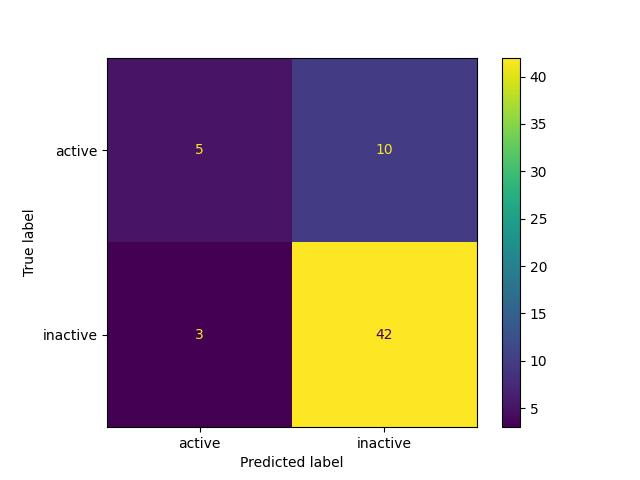
\includegraphics[height=8cm]{seh/baseline_nn_conf.jpg}
    \end{center}

\end{figure}
The proportionally high values in the diagonal(5, 42) signify good overall performance. Although the \acrshort*[]{knn} performance of \ref*{fig:seh_fe_rf_per_knn_conf} is marginally better.
\begin{figure}[H]
    \begin{center}
        \caption[]{Feature engineering permutation importance ROC curve}
        \label{fig:seh_fe_rf_per_knn_roc}
        \includegraphics[height=8cm]{seh/fe_rf_per_knn_roc.jpg}
    \end{center}

\end{figure}
An AUC of 0.67 demonstrates the model's ability to differentiate between positive and negative examples. Overall the performance is close to a random classifier.

\begin{figure}[H]
    \begin{center}
        \caption[]{Baseline neural network ROC curve}
        \label{fig:seh_baseline_nn_roc}
        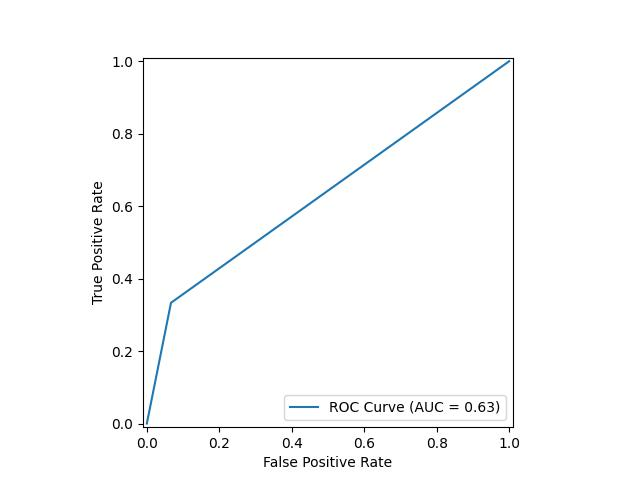
\includegraphics[height=8cm]{seh/baseline_nn_roc.jpg}
    \end{center}
\end{figure}
The ROC curve demonstrates only fair performance as it is much closer to a random classifier than it is to a perfect classifier which would be a 1.0 AUC.